
\documentclass[12pt]{report}

\usepackage{fullpage}
\usepackage{graphicx}
\usepackage{listings}
\usepackage{verbatim}
\usepackage{amsmath}
\usepackage{color}
\usepackage{hyperref}
 
\definecolor{codegreen}{rgb}{0,0.6,0}
\definecolor{codegray}{rgb}{0.5,0.5,0.5}
\definecolor{codepurple}{rgb}{0.58,0,0.82}
\definecolor{backcolour}{rgb}{0.95,0.95,0.92}
 
\lstdefinestyle{mystyle}{
    backgroundcolor=\color{backcolour},   
    commentstyle=\color{codegreen},
    keywordstyle=\color{magenta},
    numberstyle=\tiny\color{codegray},
    stringstyle=\color{codepurple},
    basicstyle=\footnotesize,
    breakatwhitespace=false,         
    breaklines=true,                 
    captionpos=b,                    
    keepspaces=true,                 
    numbers=left,                    
    numbersep=5pt,                  
    showspaces=false,                
    showstringspaces=false,
    showtabs=false,                  
    tabsize=2
}
 
\lstset{style=mystyle}
\renewcommand{\baselinestretch}{2}
\author{Mohammed Nauman Sididque}
\title{Assignment 4 \\Information Retrieval \\ CS 834 \\ Fall 2017 }

\begin{document}
\maketitle
\tableofcontents
\chapter{Problem 8.3}
\section{Problem Statement}
For one query in the CACM collection (provided at the book website), generate a ranking using Galago, and then calculate average precision, NDCG at 5 and 10, precision at 10, and the reciprocal rank by hand.
\section{Solution}
This problem uses CACM corpus provided in the test collection of the book. The queries ran against the CACM collection have been used from the processed queries section of the CACM test collection.\\

\subsection{Query: Code optimization for space efficiency}
The table below has been created manuallyby looking at the search results of the query. The first column in the table is the position in the search result,  the second column is whether the document is relevant or not and last column is the relevance score in range of 0 to 3 where 0 is for no relevance and 3 is assigned to document with high relevance.

\begin{table}[]
\centering
\caption{Relevance Table for Query:Code optimization for space efficiency }
\label{my-label}
\begin{tabular}{lll}
Index & Relevant & Relevance Score \\
1     & Yes      & 3               \\
2     & No       & 1               \\
3     & No       & 1               \\
4     & Yes      & 2               \\
5     & No       & 0               \\
6     & No       & 0               \\
7     & Yes      & 3               \\
8     & No       & 0               \\
9     & No       & 0               \\
10    & Yes      & 2              
\end{tabular}
\end{table} 

\subsubsection{ Precision}

$Precision(1) = 1/1 = 1$\\
$Precision(2) = 1/2 = 0.5$\\ 
$Precision(3) = 1/3 = 0.33$\\
$Precision(4) = 2/4 = 0.5$\\
$Precision(5) = 2/5 = 0.4$\\
$Precision(6) = 2/6 = 0.33$\\
$Precision(7) = 3/7 = 0.43$\\
$Precision(8) = 3/8 = 0.375$\\
$Precision(9) = 3/9 = 0.33$\\
$Precision(10) = 4/10 = 0.4$\\
where Precision(6) denotes precision at search result 6.\\
The precision for this query is 0.4. \\  

\subsubsection{Reciprocal Rank}
$MRR = 1/1 + 1/4 + 1/7 + 1/10$\\
$MRR = 1+ 0.25 + 0.143 + 0.1$\\
$MRR = 1.493$\\
MRR is the mean reciprocal rank for the query. For this query, the relevant results are present at position 1, 4, 7 and 10.\\
The MRR for the result is calculated to be 1.493.

\subsubsection{Normalized Discounted Cummulative Gain at 5}

Below is the list of documents D1 through D5 and their relevance scores. This data has been reused from table 1.1.\\
Documents: D1, D2, D3, D4, D5\\
Relevance Score: 3, 1, 1, 2, 0\\
$CG_5 = 3+ 1+ 1+ 2+ 0$\\
$CG_5 = 7$ \\
\begin{table}[]
\centering
\caption{Discounted Cummulative Gain}
\label{my-label}
\begin{tabular}{llll}
i & $rel_i$ & $log_2(i + 1)$   & $rel_i / log_2(i + 1)$  \\
1 & 3        & 1     		    & 3    \\
2 & 1        & 1.585 		    & 0.63 \\
3 & 1        & 2     		    & 0.5  \\
4 & 2        & 2.322 		    & 0.86 \\
5 & 0        & 2.585 		    & 0   
\end{tabular}
\end{table}
$DCG = \sum\limits_{i=1}^5 rel_i / log_2(i + 1)$ \\
$DCG = 3 + 0.63 + 0.5 + 0.86 + 0 =  4.99$\\
Ideal Discounted Cummulative Gain has the document and relevance score as below:\\
Documents: D1, D4, D2, D3, D5\\
Relevance Score: 3, 2, 1, 1, 0\\
$CG_5 = 3+ 2+ 1+ 1+ 0$\\
$CG_5 = 7$ \\
\begin{table}[]
\centering
\caption{Ideal Discounted Cummulative Gain}
\label{my-label}
\begin{tabular}{llll}
i & $rel_i$ & $log_2(i + 1)$   & $rel_i / log_2(i + 1)$  \\
1 & 3        & 1     		    & 3    \\
2 & 2        & 1.585 		    & 1.26 \\
3 & 1        & 2     		    & 0.5  \\
4 & 1        & 2.322 		    & 0.43 \\
5 & 0        & 2.585 		    & 0   
\end{tabular}
\end{table}
$IDCG = \sum\limits_{i=1}^5 rel_i / log_2(i + 1)$ \\
$IDCG = 3 + 1.26 + 0.5 + 0.43 + 0 =  5.19$\\
Normalized Discounted Cummulative Gain (NDCG)=  DCG / IDCG\\
$NDCG = 4.99 / 5.19 = 0.96$

\subsubsection{Normalized Discounted Cummulative Gain at 10}

Below is the list of documents D1 through D10 and their relevance scores. This data has been reused from table 1.1.\\
Documents: D1, D2, D3, D4, D5, D6, D7, D8, D9, D10\\
Relevance Score: 3, 1, 1, 2, 0, 0, 3, 0, 0, 2\\
$CG_{10} = 3+ 1+ 1+ 2+ 0 + 0 + 3 + 0 + 0 + 2$\\
$CG_{10}= 12$ \\
\begin{table}[]
\centering
\caption{Discounted Cummulative Gain}
\label{my-label}
\begin{tabular}{llll}
i & $rel_i$ & $log_2(i + 1)$   & $rel_i / log_2(i + 1)$  \\
1 & 3        & 1     		    & 3    \\
2 & 1        & 1.585 		    & 0.63 \\
3 & 1        & 2     		    & 0.5  \\
4 & 2        & 2.322 		    & 0.86 \\
5 & 0        & 2.585 		    & 0 \\ 
6 & 0        & 2.807     	    & 0    \\
7 & 3        & 3 		    & 1 \\
8 & 0        & 3.17    		    & 0  \\
9 & 0        & 3.22 		    & 0 \\
10 & 2      & 3.459 		    & 0.578 \\ 
\end{tabular}
\end{table}
$DCG = \sum\limits_{i=1}^{10} rel_i / log_2(i + 1)$ \\
$DCG = 3 + 0.63 + 0.5 + 0.86 + 0 + 0 + 1 + 0 + 0 + 0.578 =  6.568$\\
Ideal Discounted Cummulative Gain has the document and relevance score as below:\\
Documents: D1, D7, D4, D10, D2, D3, D5, D6, D8, D9\\
Relevance Score: 3, 3, 2, 2, 1, 1, 0, 0 , 0 , 0 \\
$CG_{10} = 3+ 3 + 2+ 2+ 1+ 1+ 0 + 0 + 0 + 0$\\
$CG_{10} = 12$ \\
\begin{table}[]
\centering
\caption{Ideal Discounted Cummulative Gain}
\label{my-label}
\begin{tabular}{llll}
i & $rel_i$ & $log_2(i + 1)$   & $rel_i / log_2(i + 1)$  \\
1 & 3        & 1     		    & 3    \\
2 & 3        & 1.585 		    & 1.89 \\
3 & 2        & 2     		    & 1  \\
4 & 2        & 2.322 		    & 0.86 \\
5 & 1        & 2.585 		    & 0.387 \\ 
6 & 1        & 2.807     	    & 0.356    \\
7 & 0        & 3 		    & 0 \\
8 & 0        & 3.17    		    & 0  \\
9 & 0        & 3.22 		    & 0 \\
10 & 0      & 3.459 		    & 0 \\ 
\end{tabular}
\end{table}
$IDCG = \sum\limits_{i=1}^{10} rel_i / log_2(i + 1)$ \\
$IDCG = 3 + 1.89 + 1 + 0.86 + 0.387 + 0.356 + 0 + 0 + 0 + 0 =  7.493$\\
Normalized Discounted Cummulative Gain (NDCG)=  DCG / IDCG\\
$NDCG = 6.568 / 7.493 = 0.977$

\chapter{Problem 8.4}
\section{Problem Statement}
For two queries in the CACM collection, generate two uninterpolated recall precision graphs, a table of interpolated precision values at standard recall levels, and the average interpolated recall-precision graph.
\section{Solution}
This problem uses CACM corpus provided in the test collection of the book. The queries ran against the CACM collection have been used from the processed queries section of the CACM test collection.\\
\subsection{Query: Code optimization for space efficiency}

\begin{table}[]
\centering
\caption{Relevance table for Query: Code optimization for space efficiency}
\label{my-label}
\begin{tabular}{ll}
index & relevant \\
1     & yes      \\
2     & no       \\
3     & no       \\
4     & yes      \\
5     & no       \\
6     & no       \\
7     & yes      \\
8     & no       \\
9     & no       \\
10    & yes     
\end{tabular}
\end{table}


\begin{table}[]
\centering
\caption{Precision and Recall Table for Query:  Code optimization for space efficiency}
\label{my-label}
\begin{tabular}{lllllllllll}
Index     & 1    & 2    & 3    & 4   & 5   & 6    & 7     & 8     & 9    & 10  \\
Relevant  & yes  & no   & no   & yes & no  & no   & yes   & no    & no   & yes \\
Recall    & 0.25 & 0.25 & 0.25 & 0.5 & 0.5 & 0.5  & 0.75  & 0.75  & 0.75 & 1   \\
Precision & 1.0  & 0.5  & 0.33 & 0.5 & 0.4 & 0.33 & 0.429 & 0.375 & 0.33 & 0.4
\end{tabular}
\end{table}

\subsection{Query: Parallel algorithms}

\begin{table}[]
\centering
\caption{Relevance table for Query:  Parallel algorithms}
\label{my-label}
\begin{tabular}{ll}
index & relevant \\
1     & no       \\
2     & yes      \\
3     & yes      \\
4     & yes      \\
5     & yes      \\
6     & yes      \\
7     & no       \\
8     & yes      \\
9     & yes      \\
10    & no      
\end{tabular}
\end{table}

\begin{table}[]
\centering
\caption{Precision and Recall Table for Query: Parallel algorithms }
\label{my-label}
\begin{tabular}{lllllllllll}
Index     & 1   & 2     & 3     & 4     & 5     & 6     & 7     & 8     & 9    & 10  \\
Relevant  & no  & yes   & yes   & yes   & yes   & yes   & no    & yes   & yes  & no  \\
Recall    & 0.0 & 0.143 & 0.286 & 0.429 & 0.571 & 0.714 & 0.714 & 0.857 & 1    & 1   \\
Precision & 0.0 & 0.5   & 0.67  & 0.75  & 0.8   & 0.833 & 0.714 & 0.75  & 0.78 & 0.7
\end{tabular}
\end{table}

\begin{figure}[ht]
  \centering
  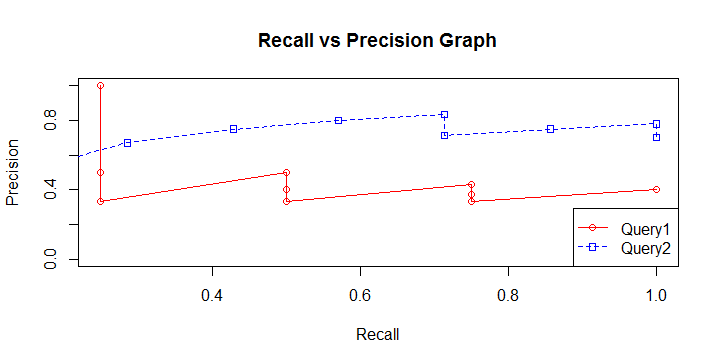
\includegraphics[width=1\textwidth]{Problem8_4/RecallvsPrecision.png}
  \caption{Recall vs Precision Graph}
  \label{fig:1}
\end{figure} 

\begin{figure}[ht]
  \centering
  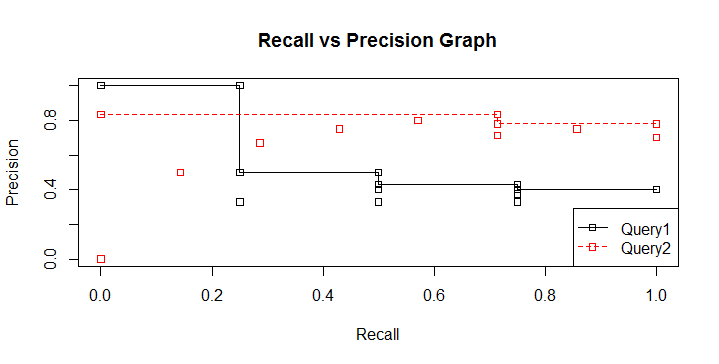
\includegraphics[width=1\textwidth]{Problem8_4/InterpolatedRecallvsPrecision.png}
  \caption{Interpolated Recall vs Precision Graph}
  \label{fig:1}
\end{figure}

\begin{table}[]
\centering
\caption{Precision values at standard recall levels calculated using interpolation}
\label{my-label}
\begin{tabular}{llllllllllll}
Recall          & 0.0   & 0.1   & 0.2   & 0.3   & 0.4   & 0.5   & 0.6   & 0.7   & 0.8  & 0.9  & 1    \\
Ranking 1       & 1     & 1     & 1     & 0.5   & 0.5   & 0.5   & 0.429 & 0.429 & 0.4  & 0.4  & 0.4  \\
Ranking 2       & 0.833 & 0.833 & 0.833 & 0.833 & 0.833 & 0.833 & 0.833 & 0.833 & 0.78 & 0.78 & 0.78 \\
Average Ranking & 0.917 & 0.917 & 0.917 & 0.667 & 0.667 & 0.667 & 0.631 & 0.631 & 0.59 & 0.59 & 0.59
\end{tabular}
\end{table}

\begin{figure}[ht]
  \centering
  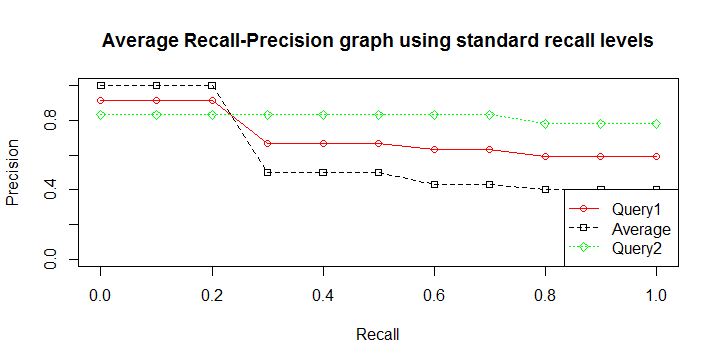
\includegraphics[width=1\textwidth]{Problem8_4/Averagerecallprecision.png}
  \caption{Average recall-precision graph using standard recall levels}
  \label{fig:1}
\end{figure}

\chapter{Problem 8.9}
\section{Problem}
For one query in the CACM collection, generate a ranking and calculate BPREF. Show that the two formulations of BPREF give the same value.
\section{Solution}
The solution is based on relevance results for query, code optimization for space efficiency. The Table 4.1 shows the relevance results for the query. The relevance results show the search results had 4 relevant documents and 6 non- relevant documents. 

\begin{table}[]
\centering
\caption{Relevance table for Query: Code optimization for space efficiency}
\label{my-label}
\begin{tabular}{ll}
index & relevant \\
1     & yes      \\
2     & no       \\
3     & no       \\
4     & yes      \\
5     & no       \\
6     & no       \\
7     & yes      \\
8     & no       \\
9     & no       \\
10    & yes     
\end{tabular}
\end{table}

\subsection{Calculating BPREF}

$BPREF = 1/R \sum\limits_{d_r}^{}(1- ({N_{d_r}} / R))$

where R is the number of non-relevant documents that are considered\\
$d_r$ is the number of relevant documents\\
 
For a query result with 4 relevant documents R is 4 implying that first 4 non-relevant documents are considered. The relevance table for the query is manipulated for BPREF as,\\

\begin{table}[]
\centering
\caption{Relevance table showing R relevant and non-relevant documents}
\label{my-label}
\begin{tabular}{ll}
Index & Relevance \\
1     & Yes       \\
2     & No        \\
3     & No        \\
4     & Yes       \\
5     & No        \\
6     & No        \\
7     & Yes       \\
10    & Yes      
\end{tabular}
\end{table}
$BPREF = 1/R \sum\limits_{d_r}^{}(1- ({N_{d_r}} / R))$\\
$BPREF = 1/4[(1-0/4) + (1 - 2/4) + (1- 4/4) + (1- 4/4)]$\\
$BPREF = 1/4 [1 + (1/2) + 0 + 0] = 3/8 = 0.375$

\subsection{Calculating BPREF based on preference}

$BPREF = P /( P + Q)$\\
where P is the number of relevant documents \\
          Q is the number of non-relevant documents\\
For query: Code optimization for space efficiency\\
P = 4\\
Q = 6\\
$BPREF = 4/(4+6)$\\
$BPREF = 0.4$\\

The value of BPREF is 0.375 and 0.4 by computing respectively with relevant documents formula and the clickthrough preference formula.
\chapter{Problem 9.8}
\section{Problem}
Cluster the following set of two-dimensional instances into three clusters using each of the five agglomerative clustering methods:
(–4, –2), (–3, –2), (–2, –2), (–1, –2), (1, –1), (1, 1), (2, 3), (3, 2), (3, 4), (4, 3)
Discuss the differences in the clusters across methods. Which methods produce the same clusters? How do these clusters compare to how you would manually cluster the points?
\section{Solution}
The code for agglomerate clustering methods generates 3 clusters for the data set.
\subsection{Discussion of the Methods}
Single Linkage: It uses the minimum distance between between elements of two clusters to merge them as one cluster. For two clusters A and B, it finds the minimum euclidean distance between the points of each cluster and compares them against the minimum threshold distance of all the other clusters to merge them in one cluster. The disadvantage of this approach is that it does not consider how far spread each cluster is and focusing only on the minimum distance between the clusters to merge them.\\ \\
Complete Linkage: It uses the maximum distance between elements of two clusters to merge them as one cluster. For two clusters A and B, it finds the maximum euclidean distance between the points of each cluster and compares them against the minimum distance of all the other clusters to merge them in one cluster. This approach creates a more comapact and less spread cluster than single linkage clustering technique.\\ \\
Average Clustering: It uses average distance of all the elements between two clusters to merge them as one cluster. For two clusters A and B, it finds the average distance by calculating the euclidean distance between all the points in each cluster and dividing them by the number of elements  in each cluster. The average distance calculated is compared against average distance of other clusters to merge the minimum average distance clusters in to one cluster. The type of cluster formed by average linkage depend heavily on the structure of clusters, since it is based on the average distance between all the elements in the two clusters. \\ \\
Average Group Clustering: It uses centroid distance between teo clusters to merge them as one cluster. For two clusters A and B, it finds the centroid of the two clusters and merges them together by comparing against the centroid distances of other clusters. It forms similar clusters to the average linkage clusters.\\ \\
Ward's Method: It uses sum of variance between two clusters to merge them as one cluster.It forms minimum spread clusters around the centroid of the cluster.\\
\lstinputlisting[language=Python]{Problem9_8/Clustering.py}
\verbatiminput{Problem9_8/ClusteringOutput.txt}
\subsection{Clustering Results vs Mannual Clustering }
All the agglomerate clustering techniques except for complete linkage technique produced the same result for the provided dataset. The results of the clusters formed by all the clustering methods has been shown above.\\
Mannual Clustering of the data points on euclidean distance results in the same clusters generated by agglomerative clustering.\\
Cluster 1: (-4,-2), (-3,-2), (--2,-2), (-1,-2)\\
Cluster 2: (1,-1), (1,1)\\
Cluster 3: (2,3), (3,2), (3,4), (4,3)\\
Cluster 1 is easy to create due to it being far away from other data points. Cluster 2 and 3 have a close margin where the distance between point (1,1) and (-1,1) is equal to 2 and the distance between point (1,1) and (2,3) is $\sqrt{5}$. Therefore the points (1,1) and (-1,1) have been clustered together as Cluster 2.\\
If the data points are clustered on the basis of the quadrants they lie in:\\
Cluster 1: 1st Quadrant$ ->$ (-4,-2), (-3,-2), (--2,-2), (-1,-2)\\
Cluster 2: 3rd Quadrant$ ->$ (1,-1)\\
Cluster 3:  4th Quadrant$ ->$ (1,1), (2,3), (3,2), (3,4), (4,3)\\
\chapter{9.9}
\section{Problem}
Use K-means and spherical K-means to cluster the data points in Exercise 9.8. How do the clusterings differ?
\section{Solution}
\lstinputlisting[language=Python]{Problem9_9/KMeans.py}
\verbatiminput{Problem9_9/Kmeans.txt}
The output of the code shows clusters on the basis of the index of data points and center of each cluster.Table 5.1 shows the index to data point relationship.The results for cluster size 2,3 and 4 are show for both the clustering techniques.\\
\begin{table}[]
\centering
\caption{Index  to Data Point relation}
\label{my-label}
\begin{tabular}{lllllllllll}
Index      & 0        & 1       & 2       & 3       & 4      & 5     & 6     & 7     & 8     & 9     \\
Data Point & (-4, -2) & (-3,-2) & (-2,-2) & (-1,-2) & (1,-1) & (1,1) & (2,3) & (3,2) & (3,4) & (4,3)
\end{tabular}
\end{table}
The clusters formed by K-means for cluster size 3 are same as the clusters formed by Single Linkage, Average Linkage and Average Group Linkage from the problem 9.8. The clusters formed by spherical K-means for cluster 3 is different from K-means due to the difference between finding similarity between points for clustering. K-means uses euclidean distance to find similarity while spherical K-mean uses cosine similarity to cluster items together. Spherical K-means clusters items on which fall in the ame quadrant approach discussed in the previous problem.\\
\chapter{Problem 9.11}
\section{Problem}
The K nearest neighbors of a document could be represented by links to those documents. Describe two ways this representation could be used in a search application.
\section{Solution}
The primary advantage of K nearest neighbor comapared to K means and agglomerative clustering techniques is that a document can be present in multiple clusters unlike the K means and agglomerative clustering technique where each documents is in a single cluster.\\

The K nearest neighbors of a documents can be used for tell-text search in search application. All the documents in the corpus can be clustered by K nearest neighbour. The document can be in multiple clusters based on the features extracted from the cluster. For a corpus of documents containing sports news from USA, it can be classified into multiple clusters as football, baseball, basketball, athletics, Olympics, CONCAF Cup etc. A document that is in cluster soccer can simultaneously be clustered with Olympics and CONCAF Cup. Similarly the queries to the documents can also be clustered on the basis of its features. It presents all the documents that are in the cluster soccer for a query of feature soccer. The same set of documents can also be recalled if the query is about CONCAF Cup. It allows for relavant search results.\\

The K nearest neighbors can also be used for showing clustered search results. It can be helped to refine a very generic query to a more precise query to return relevant result. For example, a system that employs K nearest neighbor clustering on its queries. For a user input query apple, it will show all the possible clusters where the query term apple appears. For apple, it can be a fruit, it can be the company Apple, it can be products of Apple Company etc. A user on the basis of suggestions can select the particular suggestion  to find search results that fall under the specified feature cluster.\\ 
  
   
   




  


\end{document}